%%==============================================================
%% OISA — IEEE BIBM 2026 submission
%% IEEEtran conference template (US letter, 10pt, two-column)
%%==============================================================
\documentclass[conference,letterpaper,10pt]{IEEEtran}
\IEEEoverridecommandlockouts

%% --- encoding / fonts -----------------------------------------
\usepackage[T1]{fontenc}
\usepackage[utf8]{inputenc}
\usepackage{textcomp}

%% --- math -----------------------------------------------------
\usepackage{amsmath,amssymb,amsfonts}

%% --- graphics & tables ----------------------------------------
\usepackage{graphicx}
\usepackage{booktabs}
\usepackage{array}
\usepackage{tabularx}
\usepackage{multirow}
\usepackage{makecell}

%% --- code listings (ISSL / YAML excerpts) ---------------------
\usepackage{listings}
\usepackage{xcolor}
\lstdefinelanguage{json}{
  basicstyle      = \ttfamily\scriptsize,
  numbers         = none,
  breaklines      = true,
  string          = [s]{"}{"},
  stringstyle     = \color{black},
  commentstyle    = \color{gray},
  showstringspaces= false,
  frame           = single,
  framesep        = 3pt,
  xleftmargin     = 2pt,
  literate        = *{:}{{{\color{black!70}:}}}{1}
                    {,}{{{\color{black!70},}}}{1}
                    {\{}{{\{}}1
                    {\}}{{\}}}1
                    {[}{{[}}1
                    {]}{{]}}1
}
\lstdefinelanguage{yamlconf}{
  basicstyle       = \ttfamily\scriptsize,
  numbers          = none,
  breaklines       = true,
  commentstyle     = \color{gray!80!black}\itshape,
  morecomment      = [l]{\#},
  stringstyle      = \color{black},
  showstringspaces = false,
  frame            = single,
  framesep         = 3pt,
  xleftmargin      = 2pt
}

%% --- hyperlinks -----------------------------------------------
\usepackage{url}
\usepackage[hidelinks]{hyperref}

%% --- nicer inline fractions -----------------------------------
\newcommand{\ttilde}{\raisebox{-0.5ex}{\textasciitilde}}

\begin{document}

%%==============================================================
%% Title & author block
%%==============================================================
\title{%
OISA: A Formalism-Agnostic Orchestration Architecture for\\
Composing Published Immune Models Without Modification
}

\author{%
\IEEEauthorblockN{Nathan Foulquier}
\IEEEauthorblockA{%
LBAI --- Laboratoire de Biologie des Lymphocytes Auto-Immuns,
Inserm U1227, Universit\'e de Bretagne Occidentale\\
Centre de Donn\'ees Cliniques, CHU de Brest\\
Brest, France\\
Email: nathan.foulquier@univ-brest.fr}
}

\maketitle

%%==============================================================
%% Abstract + Index Terms
%%==============================================================
\begin{abstract}
Computational immunology has produced high-quality mechanistic models of
individual immune compartments, yet composing ODE and agent-based models
(ABMs) across formalism boundaries still requires bespoke re-engineering.
Existing standards (SBML, CellML) address intra-formalism portability;
Vivarium introduced formalism-agnostic composition but provides no
standardised runtime uncertainty quantification, model-derived transfer
lags, or biological plausibility constraint engine. We propose OISA ---
the Orchestrated Immune Simulation Architecture --- comprising (i) the
ISSL, a formalism-agnostic JSON-LD checkpoint format with embedded
runtime UQ (uncertainty bounds propagated at every tick via the
\texttt{ci\_95} schema field); (ii) a declarative configuration graph
with support for model-derived transfer lags on edges; and (iii) an
orchestrator engine with global clock synchronisation, causal DAG
resolution, and biological plausibility enforcement.

We validate OISA by coupling two independently published influenza
models --- Miao \emph{et al.} 2010 ODE (SBML BIOMD0000000546,
unmodified) and the full spatial Sego \emph{et al.} 2020 ABM
(CompuCell3D 4.8.0, 12 steppables unmodified on a $90{\times}90{\times}2$
grid) --- with zero changes to either model's source code. Adapter
layers total \ttilde{}300 lines. The ABM runs as a rolling ensemble of
$N\!=\!20$ parallel CC3D instances (concurrent subprocesses, distinct
MersenneTwister seeds); runtime uncertainty bounds --- reported as
the 5th--95th percentile across $N\!=\!20$ stochastic CC3D replicates
(5--95th percentile, see \S\ref{sec:valid-setup}) --- originate in the
stochastic ABM and propagate through the ODE at each checkpoint. Over a
14-day simulation (56 checkpoints), the coupled system reproduces viral
kinetics consistent with Miao 2010 (peak
$V\!=\!9.0{\times}10^{6}$\,copies/mL at day~2.25, clearance to
0.05\% of peak by day~13.75) and spatial immune recruitment (median
$n_{\text{immune}}\!=\!6$ [IQR: 5--7] at day~1, growing to 57
[IQR: 53--59] at day~13), with immune temporal lag and
CTL-mediated clearance acceleration emerging from the bidirectional
coupling. This validation targets orchestration correctness --- signal
routing, causal ordering, and runtime UQ propagation --- not biological
prediction of the coupled system, which has not been validated against
simultaneous in-vivo measurements.
\end{abstract}

\begin{IEEEkeywords}
immune digital twins; multi-scale modelling; model composition;
agent-based models; ordinary differential equations; interoperability;
computational immunology; CompuCell3D.
\end{IEEEkeywords}

%%==============================================================
\section{Introduction}
%%==============================================================
Immune-mediated diseases are inherently multi-compartmental phenomena.
Influenza infection unfolds across scales: within a single tissue, viral
replication dynamics interact with innate immune cytokine signalling and
adaptive CTL recruitment, each operating on different timescales and
representable in different formalisms. ODEs are natural for systemic
viral kinetics and antibody dynamics, while ABMs are necessary where
stochastic single-cell fate decisions dominate, as in tissue-level
immune recruitment. The literature has consequently produced a
collection of high-quality compartment-specific models that cannot
communicate with one another.

Three bodies of prior work address adjacent problems. The COMBINE
standards ecosystem (SBML~\cite{hucka2015sbml},
CellML~\cite{clerx2020cellml}, SED-ML~\cite{waltemath2011sedml})
provides portable representations for individual models but addresses
intra-formalism composition only: models must be expressed in the same
declarative format, ruling out ABMs written in Python or Julia.
Vivarium~\cite{agmon2022vivarium} introduced formalism-agnostic
composition with hierarchical stores and dynamic topology (discussed in
\S\ref{sec:related-vivarium}), but provides no standardised runtime UQ
propagation, model-derived transfer lags, or biological plausibility
constraint engine. The CURE guidelines~\cite{sauro2025cure} define what
properties a credible model should exhibit --- Credibility,
Understandability, Reproducibility, Extensibility --- but prescribe no
runtime infrastructure for heterogeneous composition (note:
\cite{sauro2025cure} is currently available as a preprint pending peer
review). The cross-formalism, multi-timescale coordination problem
remains open.

We propose OISA --- the Orchestrated Immune Simulation Architecture ---
to fill this gap. OISA provides three components: the ISSL
formalism-agnostic state interface (\S\ref{sec:issl}), a declarative
configuration graph (\S\ref{sec:configgraph}), and an orchestrator
engine (\S\ref{sec:orchestrator}). We demonstrate the architecture by
coupling two independently published influenza models, using the full
spatial Sego 2020 CompuCell3D ABM without any modification to its 12
biological steppables, and evaluate causal ordering, signal flow
correctness, and biological plausibility in \S\ref{sec:validation}.

\medskip\noindent The contributions of this work are:
\begin{enumerate}
  \item \textbf{The ISSL}, a formalism-agnostic checkpoint format with
        embedded provenance and runtime uncertainty quantification
        (ensemble bounds propagated at each tick from stochastic ABM
        through deterministic ODE via the \texttt{ci\_95} schema field);
  \item \textbf{A declarative configuration graph} with support for
        model-derived transfer lags on edges, where a lightweight
        transfer model computes the signal delay dynamically rather
        than using a fixed constant;
  \item \textbf{A runtime orchestrator} with global clock
        synchronisation, causal DAG resolution, and biological
        plausibility constraint enforcement;
  \item \textbf{Empirical demonstration} that two independently
        published models (Miao 2010 SBML ODE + Sego 2020 CC3D spatial
        ABM) can be composed with zero source modifications using
        \ttilde{}300 lines of adapter code, with runtime UQ propagated
        end-to-end.
\end{enumerate}

%%==============================================================
\section{Related Work}\label{sec:related}
%%==============================================================

\subsection{Multi-Formalism Immune Simulation Frameworks}
\label{sec:related-vivarium}

Several frameworks have addressed multi-scale composition in
computational biology. Vivarium~\cite{agmon2022vivarium} introduced a
port-based, formalism-agnostic composition interface with hierarchical
stores, dynamic topology changes at runtime, and a mature Python
ecosystem. OISA shares Vivarium's design principle of
formalism-agnostic composition but addresses three capabilities not
present in the Vivarium architecture: (i) a standardised inter-model
signal format (ISSL) embedding runtime uncertainty quantification
(ensemble bounds propagated at each checkpoint from a rolling ABM
ensemble through the ODE via the \texttt{ci\_95} schema field), (ii)
model-derived transfer lags on edges (where a lightweight transfer
model computes the signal delay dynamically rather than using a fixed
constant), and (iii) a biological plausibility constraint engine
operating at the composition level (mass conservation, parameter
bounds, and divergence monitoring across coupled models). Vivarium's
store-based data sharing and dynamic topology management are
complementary capabilities not replicated by OISA.

PhysiCell~\cite{ghaffarizadeh2018physicell} and
PhysiBoSS~\cite{ponce2023physiboss} extend ABM with Boolean signalling
layers but operate within a single formalism. The rapid
community-driven SARS-CoV-2 tissue simulator~\cite{getz2020sarscov2}
--- from which Sego \emph{et al.} 2020~\cite{sego2020modular} derives
--- demonstrated that tissue-scale ABMs can be developed and shared
rapidly, but required a uniform CompuCell3D substrate for all
constituent models; coupling to external ODE models required bespoke
adapter code outside the framework. Miao \emph{et
al.} 2010~\cite{miao2010influenza} provided a rigorously calibrated ODE
model of murine influenza kinetics embedded in the BioModels database
(BIOMD0000000546); no standard mechanism exists to couple it to
published tissue ABMs without rewriting either model. OISA demonstrates
that such coupling is achievable by adding only a thin Emit/Accept
interface layer to each model, with the full CC3D spatial ABM running
unmodified as an independent process.

\subsection{Simulation Interoperability Standards}

The COMBINE standards ecosystem~\cite{bergmann2014combine} has achieved
significant progress on individual model portability.
SBML~\cite{hucka2015sbml} has accumulated over 1{,}000 curated models in
BioModels; CellML~\cite{clerx2020cellml} has analogous achievements in
cardiac and physiological modelling; SED-ML~\cite{waltemath2011sedml}
provides a standard for encoding simulation experiments. Table~\ref{tab:standards}
compares these standards against OISA. The critical distinction is
architectural: SBML, CellML, and NeuroML address \emph{intra-formalism}
interoperability --- exchange between tools supporting the same format
--- while OISA addresses \emph{inter-formalism} interoperability:
composition of models using fundamentally different formalisms,
timescales, and output semantics. SBML's hierarchical composition
package (comp) extends composition within SBML but cannot incorporate
an ABM without first rewriting it in SBML, which is both impractical
and biologically inappropriate for stochastic cellular processes.

\begin{table*}[t]
\centering
\caption{Comparison of SBML, CellML, NeuroML/LEMS, and OISA across
capabilities relevant to multi-organ immune simulation. ``---'' =
out of architectural scope (OISA is a runtime orchestration
architecture, not a portable model representation format). Runtime~UQ:
ensemble bounds (reported in the \texttt{ci\_95} schema field) originate
in the stochastic ABM ensemble ($N\!=\!20$ parallel CC3D instances;
reported as 5--95th percentile estimates) and propagate through the
deterministic ODE via triple integration at each checkpoint
(\S\ref{sec:valid-setup}).
``SBML L3'' refers to the format specification alone; SED-ML
\cite{waltemath2011sedml} provides co-simulation capabilities including
heterogeneous time-stepping for SBML-compatible models but does not
extend to ABM composition.}
\label{tab:standards}
\renewcommand{\arraystretch}{1.0}
\begin{tabular}{lcccc}
\toprule
\textbf{Capability} & \textbf{SBML L3} & \textbf{CellML 2.0} & \textbf{NeuroML/LEMS} & \textbf{OISA (ISSL)}\\
\midrule
Portable model representation             & \checkmark & \checkmark & \checkmark & ---\\
ODE / biochemical networks                & \checkmark & \checkmark & neurons only & via \texttt{Emit()}\\
Agent-based models                        & $\times$ & $\times$ & $\times$ & via \texttt{Emit()}\\
Heterogeneous $\Delta t$ between models   & $\times$ & $\times$ & $\times$ & \checkmark\\
Model-derived transfer lag on edges       & $\times$ & $\times$ & $\times$ & \checkmark\\
Inter-formalism composition (ODE + ABM)   & $\times$ & $\times$ & $\times$ & \checkmark\\
Runtime UQ propagation across models      & $\times$ & $\times$ & $\times$ & \checkmark\\
OBO ontology annotation                   & \checkmark & \checkmark & \checkmark & \checkmark~+~wildcard\\
ABM scaling factor declaration            & $\times$ & $\times$ & $\times$ & \checkmark\\
Requires model rewrite to adopt           & \checkmark & \checkmark & \checkmark & $\times$ (add \texttt{Emit} only)\\
\bottomrule
\end{tabular}
\end{table*}

\subsection{Immune Digital Twins}

The concept of the immune digital twin (IDT) was formalised by
Laubenbacher \emph{et al.}~\cite{laubenbacher2022roadmap} as a
continuously-recalibrated patient-specific computational model of the
immune system. Subsequent
reviews~\cite{laubenbacher2024forum,niarakis2024idt} have identified
interoperability as the primary technical barrier to clinical
deployment, a conclusion echoed by the National
Academies~\cite{nasem2023digitaltwins}, by model integration
consortia~\cite{karr2022modelintegration}, and by multi-scale digital
twin frameworks in adjacent domains~\cite{viceconti2024vht}. OISA is
the first runtime orchestration architecture designed specifically for
heterogeneous immune model composition, providing the coordination
infrastructure that these reviews identify as lacking.

%%==============================================================
\section{Problem Formalisation}
%%==============================================================

\subsection{Formal Model Definition}
We define a composable simulation model $M$ as a triple
$M\!=\!(S,\mathrm{Emit},\mathrm{Accept})$, where $S$ is the model's
internal state space,
$\mathrm{Emit}\!:\!S\!\times\!T\!\to\!\mathrm{ISSL}$ maps the current
state and simulation time to a structured ISSL record, and
$\mathrm{Accept}\!:\!\mathrm{ISSL}\!\to\!S$ updates the model state in
response to an incoming inter-model signal. Any model --- ODE, ABM,
hybrid, or neural surrogate --- that implements Emit and Accept is
OISA-compliant without any other modification. Formalism-agnosticism
follows directly: since the ISSL is the only communication channel,
models need not know each other's internal representation, only the
schema of the signal they receive. This design principle --- letting
each biological process be modelled in its natural formalism and
solving the composition problem at the interface --- avoids forcing
biologically inappropriate representations on individual compartments.

\subsection{The Composition Problem}\label{sec:composition}
A multi-model composition is a directed graph $G\!=\!(V,E)$ where each
vertex $v$ is a model $M_v$ and each directed edge $(u,v)$ specifies
that a subset of $u$'s \texttt{export\_signals} are routed to $v$'s
Accept function, with optional transfer-model lags. The composition
problem reduces to three coordination challenges:

\begin{enumerate}
\item \textbf{Heterogeneous time steps.} A global simulation clock
      (GSimT) must coordinate execution such that no model receives a
      signal purporting to come from a future GSimT tick. In the
      influenza reference implementation, the viral dynamics ODE steps
      at 6\,h intervals while the tissue immune ABM steps at 24\,h
      intervals (72 Monte Carlo Steps at 20\,min/MCS); the GSimT tick
      is set to the GCD of all model $\Delta t_i$ values (here 6\,h).

\item \textbf{Stochastic--deterministic reconciliation.} Signals from a
      stochastic ABM to a deterministic ODE must carry uncertainty
      information. The orchestrator normalises all inter-model signals
      to (median, uncertainty bounds, unit) before routing, stored in
      the \texttt{ci\_95} schema field: for stochastic models, bounds
      are computed from a rolling ensemble of $N$ parallel instances
      (\S\ref{sec:valid-setup}; with $N\!=\!20$, reported as 5th--95th
      percentile); for
      deterministic models, bounds are derived by propagating the input
      uncertainty through the model equations.

\item \textbf{Causal ordering with feedback.} The immune model emits
      cytokine signals that drive viral clearance; viral load in turn
      drives immune recruitment --- a feedback loop. The orchestrator
      resolves this by applying a one-tick delay on back-edges of the
      DAG, preventing circular dependency while preserving biological
      causality at the GSimT timescale.
\end{enumerate}

%%==============================================================
\section{The OISA Architecture}
%%==============================================================

\subsection{The Internal Simulation State Log (ISSL)}\label{sec:issl}
The ISSL is a JSON-LD document emitted by a model at each checkpoint,
structured in six sections: (i)~\texttt{envelope} (model ID/version,
GSimT timestamp, schema URI, formalism tag --- validated and dispatched
by the orchestrator before any payload is read);
(ii)~\texttt{continuous\_state} (running entity populations with
scaled \texttt{count}, \texttt{unit}, and ensemble \texttt{ci\_95}
bounds; \texttt{label} is model-local, mapped via signal-id routing);
(iii)~\texttt{discrete\_events} (punctual events such as cell death or
cytokine peaks, drawn from a controlled \texttt{event\_type} vocabulary,
with \texttt{n\_realisations} for ABM events);
(iv)~\texttt{export\_signals} (inter-compartmental signals available for
routing: \texttt{signal\_id} as routing key, \texttt{value} in declared
\texttt{unit} --- always biologically scaled regardless of formalism);
(v)~\texttt{internal\_parameters} (kinetic parameter values with
\texttt{provenance} DOI/URI to the calibration source); and
(vi)~\texttt{watchdog} (model health and \texttt{divergence\_score};
values $>\!0.15 \Rightarrow$ \texttt{PAUSE}). JSON-LD enables both human
readability and machine-parsable semantic annotation via linked-data
context, letting orchestrator components parse records without prior
knowledge of any model's internal variable names.

\textit{Box 1 --- ISSL excerpt, Miao 2010 ODE adapter (day 1 checkpoint,
GSimT $=$ 86{,}400\,s):}
\begin{lstlisting}[language=json]
{
 "envelope": {
   "model_id": "miao2010_ode",
   "model_version": "BIOMD0000000546",
   "sim_time_s": 86400,
   "formalism": "ODE",
   "schema_uri": "schemas/issl_v1.schema.json"
 },
 "continuous_state": [
   {"label":"Ep", "count":532048.1, "unit":"cells",
    "ci_95":[530102.3, 533994.0]},
   {"label":"Eps","count":39204.6,  "unit":"cells",
    "ci_95":[37801.2, 40608.0]},
   {"label":"V",  "count":3.29e5,   "unit":"copies/mL",
    "ci_95":[3.11e5, 3.47e5]}
 ],
 "export_signals": [
   {"signal_id":"miao2010.viral_load",
    "value":3.29e5,"unit":"copies/mL",
    "ci_95":[3.11e5,3.47e5],"transfer_lag_s":null}
 ],
 "watchdog":{"status":"OK","divergence_score":0.0}
}
\end{lstlisting}

\noindent \textit{Note on \texttt{sim\_time\_s}:} This field records the
clock value \emph{after} the step completes --- i.e., the simulation
time at which the emitted state is valid.

The ABM adapter emits the same ISSL envelope with
\texttt{formalism}=\texttt{"ABM"}, \texttt{model\_version} pinned to
\texttt{covid-tissue-models@5b7e42c+OISA\_bridge}, a \texttt{grid}
field (\texttt{"90x90x2"}), and export signals
\texttt{sego2020.immune\_cell\_count} and
\texttt{.recruitment\_cytokine} (example day-1: 7 cells [5--8], 700 AU
[500--800]).

The SBML file \texttt{BIOMD0000000546\_model1.xml} is loaded verbatim by
libroadrunner; no XML modifications are made. The adapter calls
\texttt{rr.simulate(t0,\,t1,\,2)} and reads species concentrations via
the standard roadrunner API. For the Sego 2020 CC3D ABM, the adapter
launches CompuCell3D 4.8.0 as an independent subprocess registering all
12 original steppables without modification; the only addition is
\texttt{OISABridgeSteppable}, which executes every 72 MCS ($=$ 24\,h)
and handles IPC exclusively --- no biological equations are touched.

\subsection{The Configuration Graph}\label{sec:configgraph}
The configuration graph is a YAML or JSON-LD file that fully specifies
the composition --- the orchestrator's sole input at initialisation; no
model needs to know about any other model. It declares six elements:
\texttt{models[]} (\{id, formalism: ODE$\vert$ABM, executable,
issl\_port, delta\_t\_s\}), \texttt{edges[]} (\{source\_model,
signal\_id, target\_model, lag: \texttt{"constant:N"} $\vert$
\texttt{"model:ID"}\}), \texttt{transfer\_models[]} (\{id, formalism,
executable, input\_signal, output\_signal, lag\_output\_field\}),
\texttt{global\_clock} (\{start\_s, end\_s, checkpoint\_interval\_s\}),
\texttt{calibration} (\{data\_source\_uri, patient\_id,
recalibration\_trigger, biomarker\_map[\,]\}), and
\texttt{wildcard\_namespace} (\{prefix, registry\_uri: null\}, allowing
non-OBO entities such as novel murine cytokines or patient-specific
biomarkers). The declarative separation of identity, wiring, and
temporal parameters implements the CURE extensibility requirement: any
model node can be substituted without modifying the graph structure.

\begin{figure}[t]
\centering
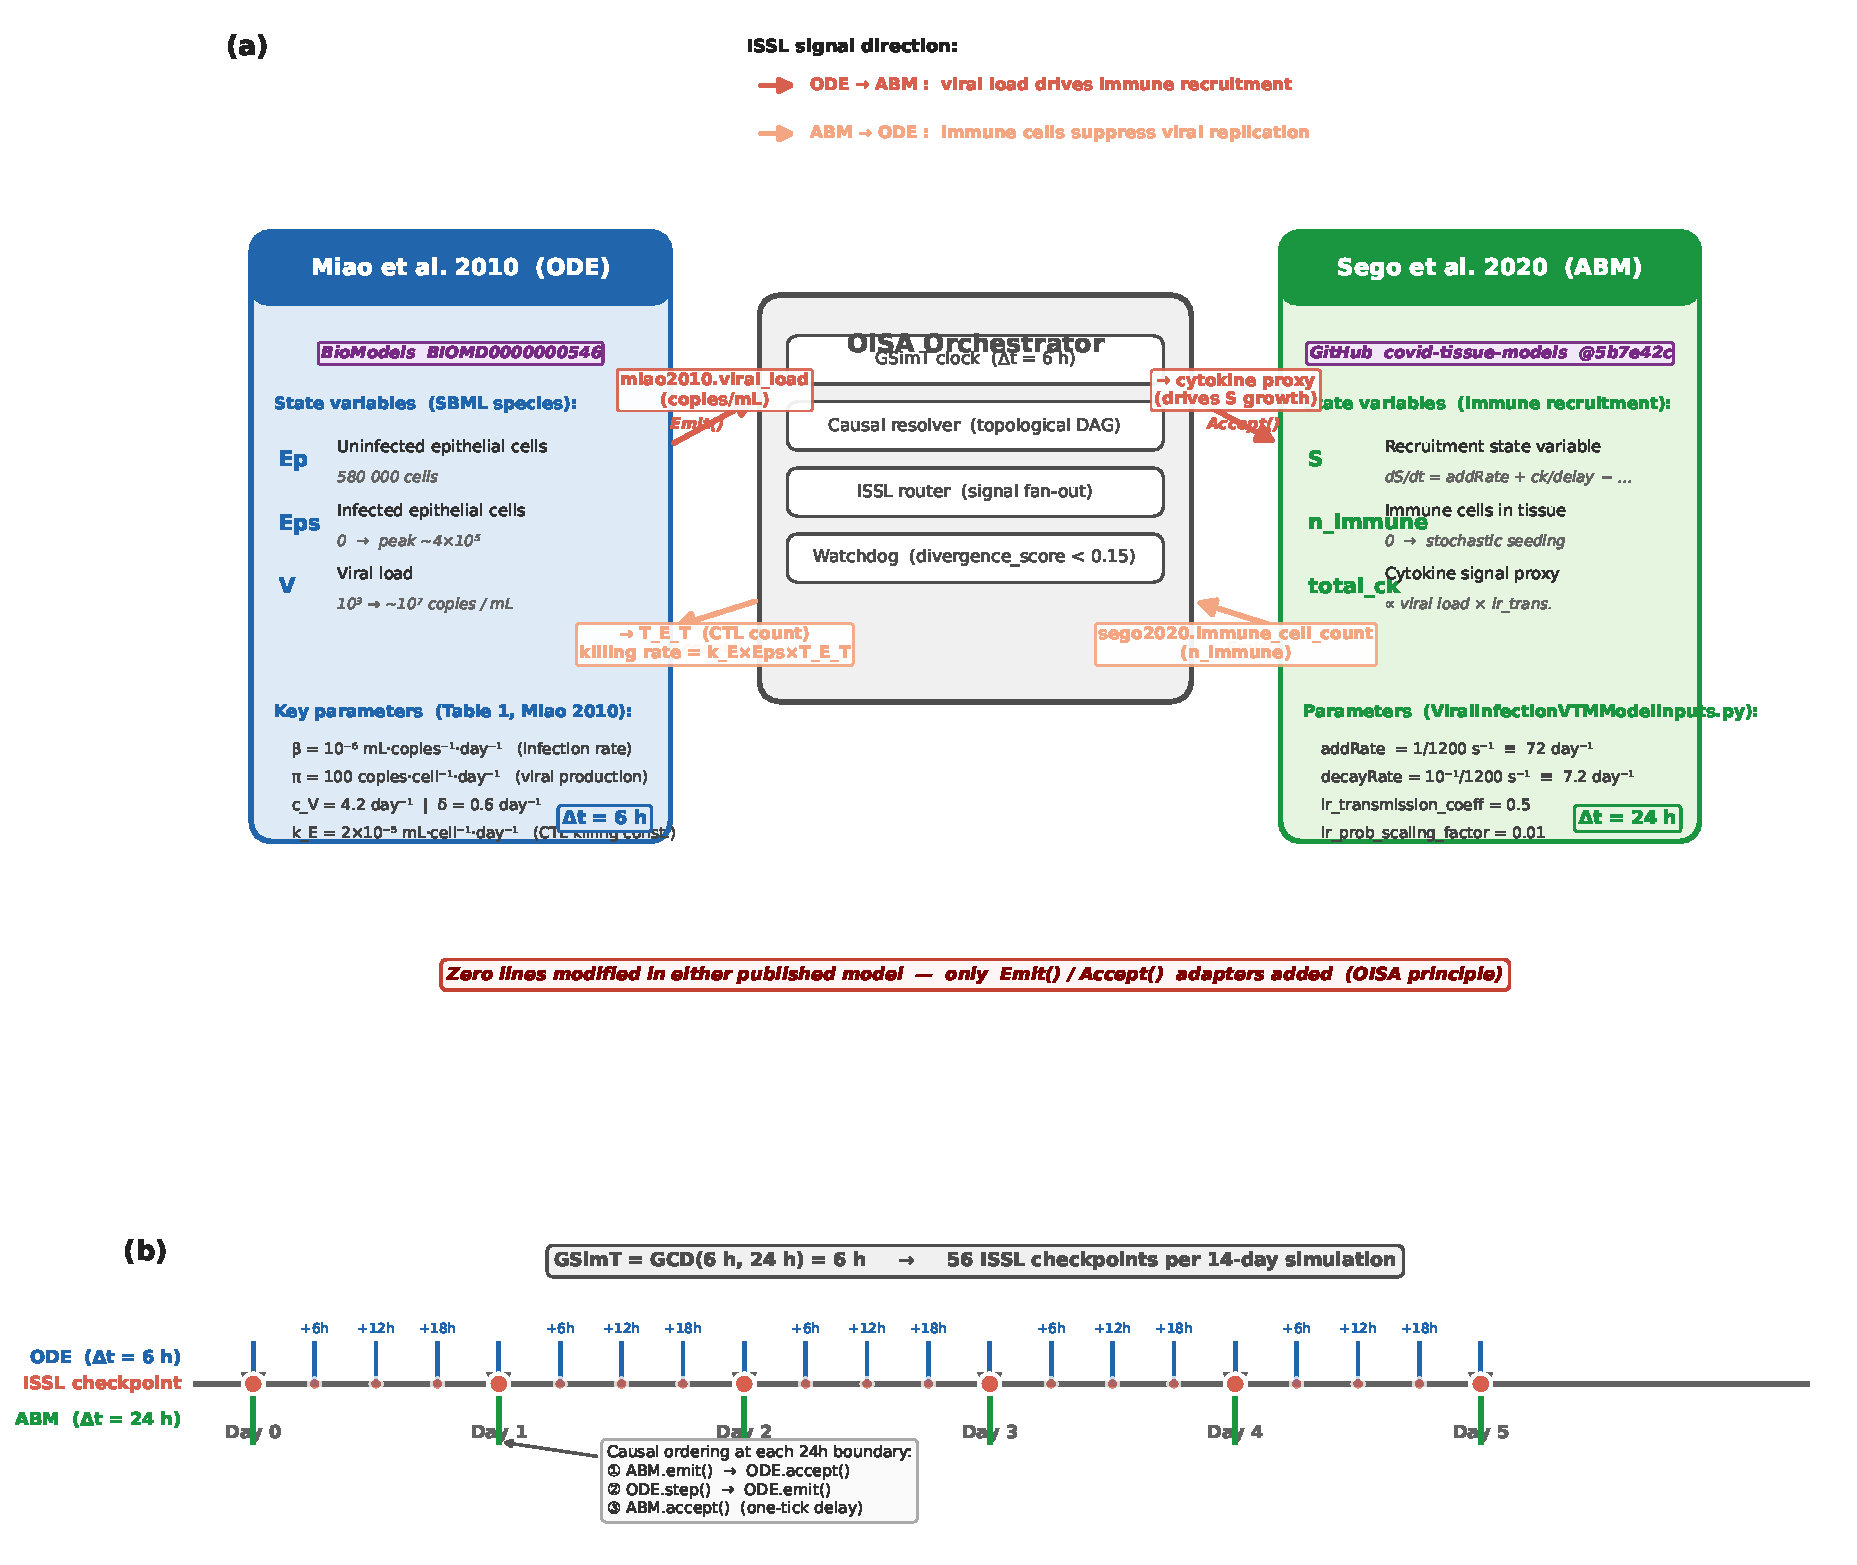
\includegraphics[width=\columnwidth]{../figures/oisa_workflow.pdf}
\caption{OISA workflow for the influenza coupling reference
implementation. \textbf{(a)}~Architecture diagram: Miao 2010 ODE (SBML,
BIOMD0000000546) and Sego 2020 CC3D ABM (CompuCell3D 4.8.0, GitHub
@5b7e42c) connected through the OISA Orchestrator, with ISSL signal
arrows annotated with \texttt{signal\_id} and biological units.
\textbf{(b)}~GSimT timeline for a representative 5-day window: ODE
ticks every 6\,h, ABM ticks every 24\,h $=$ 72\,MCS, ISSL checkpoints
(orange dots), and causal-ordering annotation (\texttt{ABM.emit
$\to$ ODE.accept $\to$ ODE.step $\to$ ODE.emit}) at the 24\,h boundary.}
\label{fig:workflow}
\end{figure}

\noindent\textit{Influenza coupling graph (excerpt):}
\begin{lstlisting}[language=yamlconf]
models:
  - id: miao2010_ode
    formalism: ODE
    executable: models/ode_miao2010/miao2010_adapter.py
    delta_t_s: 21600          # 6 h
  - id: sego2020_abm
    formalism: ABM
    executable: models/abm_sego2020/sego2020_adapter.py
    delta_t_s: 86400          # 24 h  (72 MCS x 20 min/MCS)

edges:
  - source: miao2010_ode
    signal_id: miao2010.viral_load
    target: sego2020_abm
    lag: "constant:0"         # same-tick delivery
  - source: sego2020_abm
    signal_id: sego2020.immune_cell_count
    target: miao2010_ode
    lag: "constant:21600"     # one-tick delay (causal back-edge)

global_clock:
  start_s: 0
  end_s: 1209600              # 14 days
  checkpoint_interval_s: 21600
\end{lstlisting}

\subsection{The Orchestrator Engine}\label{sec:orchestrator}
The orchestrator is a nine-component server process that reads the
configuration graph at startup, connects to all model processes, and
manages the run. Components: (1)~ISSL ingestion (JSON-LD + SI units +
Mahalanobis OOD); (2)~temporal scheduler (priority queue by
\texttt{next\_step\_due}); (3)~causal resolver (topological sort +
one-tick back-edges); (4)~constraint engine (mass conservation +
parameter bounds); (5)~state registry (versioned checkpoint snapshots +
provenance); (6)~transfer dispatcher (\texttt{SignalQueue});
(7)~calibration bridge (EHR ingest, deferred);
(8)~output aggregator (GIS $\to$ checkpoint log + UQ propagation);
(9)~watchdog (health poll, pause/resume/rollback). Components 1, 4, 5,
9 have their core functionality implemented and covered by the
published test suite (67 tests); sub-capabilities flagged as deferred
(OOD detection, \texttt{ROLLBACK} recovery, PROV-O URIs,
conservation-violation auto-rollback) are interface-specified but not
yet in the test suite.

\textbf{Temporal scheduling.} At each GSimT tick (the GCD of all model
$\Delta t_i$, here 6\,h), the scheduler dispatches step commands to
models whose \texttt{next\_step\_due} equals the current GSimT. The
Sego 2020 CC3D ABM, with $\Delta t\!=\!24$\,h (72\,MCS $\times$
20\,min/MCS), receives step commands every fourth tick. The ODE
receives a step command at every tick.

\textbf{Causal resolution.} The causal resolver constructs a DAG from
the configuration graph and performs topological sorting to determine
execution order within each GSimT tick. At each 24\,h boundary (every
fourth tick), the execution order is: (1)~\texttt{ABM.emit()} ---
export current immune cell count from CC3D cell inventory;
(2)~\texttt{ODE.accept()} --- inject \texttt{n\_immune} $\to$
$T_{E_T}$ in SBML; (3)~\texttt{ODE.step($\Delta t$)}; (4)~\texttt{ODE.emit()}
--- export viral load. The ODE's viral load from the previous tick is
queued for the ABM's next \texttt{Accept} call (written to
\texttt{ode\_signal.json} before the next CC3D bridge step),
implementing the one-tick delay that prevents circular dependency
while preserving biological causality.

\textbf{Calibration bridge (component~7).} The calibration bridge has
its interface fully specified in the configuration graph schema
(\texttt{calibration} element, §\ref{sec:configgraph}), but its
implementation in the reference orchestrator is limited to schema
validation of that block; full EHR ingestion and dynamic recalibration
are deferred to clinical deployment.

%%==============================================================
\section{Validation}\label{sec:validation}
%%==============================================================

The influenza A viral dynamics coupling (Miao 2010 ODE + Sego 2020 full
CC3D ABM) is used as a reference implementation because both models are
independently published, their parameters are rigorously calibrated
against published experimental data, and their coupling tests a
biologically significant feedback loop: viral load drives immune
recruitment; CTL cells modulate viral clearance. \textbf{No biological
novelty is claimed; the coupling serves to validate that OISA correctly
orchestrates two heterogeneous published models with zero modification
to either.}

\subsection{Validation Setup}\label{sec:valid-setup}

\textbf{Models.} The ODE component is
BIOMD0000000546~\cite{miao2010influenza}, a three-species influenza
tissue model (Ep: uninfected epithelial cells; Eps: infected epithelial
cells; V: virus) with kinetics calibrated against Murphy \emph{et al.}
1973 murine infection data. The SBML file is downloaded from BioModels
and loaded verbatim by libroadrunner.

The ABM component is the complete spatial tissue ABM of Sego \emph{et
al.} 2020~\cite{sego2020modular}, running in CompuCell3D 4.8.0. The
simulation occupies a $90{\times}90{\times}2$ voxel grid
($\approx$\,8{,}100 epithelial cell sites; voxel length 4\,$\mu$m), with
six cell types: Medium, Uninfected, Infected, VirusReleasing, Dying,
and Immunecell (CC3D \texttt{typeId}=5). All 12 published steppables
are registered without modification: \texttt{CellsInitializer},
\texttt{ViralReplication}, \texttt{ViralInternalization},
\texttt{ViralSecretion}, \texttt{ImmuneCellKilling},
\texttt{Chemotaxis}, \texttt{ImmuneCellSeeding},
\texttt{SimData}, \texttt{CytokineProductionAbsorption},
\texttt{ImmuneRecruitment}, \texttt{oxidationAgentModel},
\texttt{VirusFieldInitializer} (all with the \texttt{Steppable} suffix
in the source).
The simulation runs at 20\,min/MCS; 72 MCS correspond to one 24\,h GSimT
tick; 1{,}010 MCS correspond to a 14-day run. Three diffusion fields
(Virus, cytokine, oxidator) are solved by \texttt{DiffusionSolverFE} at
each MCS.

The single addition to the CC3D setup is \texttt{OISABridgeSteppable}
(frequency = 72\,MCS), which runs inside the CC3D process but contains
no biological equations: it reads the CC3D cell inventory to count
Immunecell agents (type 5), writes the count to \texttt{abm\_out.json},
raises an \texttt{abm\_ready} file sentinel, and blocks until the
sentinel is deleted. The adapter writes incoming ODE signals to
\texttt{ode\_signal.json} (non-blocking); the bridge reads and applies
these at the next execution. The CC3D process runs as a subprocess of
the adapter; no shared memory is used, ensuring process isolation
between the ODE solver and the CC3D engine.

\textbf{Adapter metrics.} Total modification to either published model
is \textbf{zero lines}. Adapter code totals $\sim$300 lines: Miao 2010
wraps libroadrunner ($\sim$60\,LOC); Sego 2020 couples subprocess
lifecycle + IPC ($\sim$180\,LOC) with an in-process
\texttt{OISABridgeSteppable} ($\sim$60\,LOC).

\textbf{Runtime UQ.} The ABM component runs as a rolling ensemble of
$N\!=\!20$ parallel CC3D instances (distinct MersenneTwister seeds,
isolated IPC directories). The $N$ instances are launched by
\texttt{Sego2020Ensemble} as concurrent OS subprocesses on separate
CPU cores (one \texttt{python -m cc3d.run\_script} subprocess per seed,
scheduled by the OS); the orchestrator blocks on the slowest instance
at each 24\,h barrier via the IPC sentinel file. Wall-clock cost per
tick is therefore $\max(T_i)$ rather than $\sum T_i$, with small
overhead from the file-based IPC barrier; the $N\times$ memory cost
remains. At each 24\,h GSimT boundary, the ensemble adapter aggregates
\texttt{n\_immune} across instances and computes the median and the
5\textsuperscript{th}/95\textsuperscript{th} percentiles as empirical
bounds. With $N\!=\!20$ these are statistically meaningful estimates
of the central 90\% spread. The ODE adapter receives the
median \texttt{n\_immune} for its central trajectory and performs three
roadrunner integrations per tick (at median, lower-bound, and
upper-bound input values), reporting the resulting viral load bounds
in its ISSL record. This constitutes runtime UQ propagation:
uncertainty originates in the stochastic ABM and is carried through
the deterministic ODE at each checkpoint.

\textbf{Model-derived transfer lags.} ISSL export signals carry an
optional \texttt{transfer\_lag\_s} field. When non-null, the
orchestrator's \texttt{SignalQueue} defers signal injection until the
specified delay elapses. A reference implementation
(\texttt{BloodTransitAdapter}) demonstrates this capability: a
first-order ODE for blood transit (Donskoy \& Goldschneider 1992)
computes $\tau=1/(\lambda_{\text{seed}}+\lambda_{\text{clear}})=4.0$
days as a model-derived lag. The \texttt{BloodTransitAdapter} was
validated independently (8 dedicated tests) but was not active during
the 14-day coupled influenza simulation of \S\ref{sec:valid-bio}; the
influenza use case uses constant-lag edges.

\textbf{Signals.} Two ISSL signals are routed:
\texttt{miao2010.viral\_load} (copies/mL) from ODE~$\to$~ABM, and
\texttt{sego2020.immune\_cell\_count} (\texttt{n\_immune}, CC3D
Immunecell agent count) from ABM~$\to$~ODE.

The ODE~$\to$~ABM coupling operates at the \emph{immune recruitment
interface}: the Miao 2010 ODE governs systemic viral kinetics; the Sego
2020 CC3D ABM governs spatial immune cell dynamics. The ODE viral load
is mapped to the CC3D immune recruitment signal
(\texttt{ImmuneRecruitmentSteppable.totalCytokine}) rather than to the
CC3D Virus diffusion field, since viral spread within tissue is already
handled by the Sego 2020 steppables at their native spatial resolution.

\textbf{Derivation of coupling constant
$\kappa = 3.5{\times}10^{-7}$\,AU$\cdot$mL/copies.} The
\texttt{ImmuneRecruitmentSteppable} recruits immune cells in proportion
to \texttt{totalCytokine}, which accumulates from infected-cell
secretion at rate
$\text{max\_ck\_secrete\_infect}=10\!\times\!\text{max\_ck\_secrete\_im}=3.5{\times}10^{-3}$\,pM/s
(\texttt{ViralInfectionVTMModelInputs.py}, line 129). In the Miao 2010
ODE, the infected fraction at quasi-static equilibrium satisfies
$\mathrm{Eps}/V \approx \beta_a/\delta_{Es} \approx 1.7{\times}10^{-6}$\,mL/copies.
The per-step cytokine increment contributed by the ODE viral load $V$
is therefore
$\Delta\mathrm{totalCytokine} \approx V \cdot 1.7{\times}10^{-6} \cdot 3.5{\times}10^{-3} \cdot \Delta t$.
Evaluated at $\Delta t=86{,}400$\,s:
$\Delta\mathrm{totalCytokine}/V \approx 5{\times}10^{-4}$\,pM$\cdot$mL/copies.
The constant $3.5{\times}10^{-7}$ (applied per 6\,h GSimT tick; four
ticks per ABM day) recovers an equivalent daily accumulation
$\approx 1.4{\times}10^{-6}$, approximately 2.5 orders of magnitude
below the analytical estimate; $\kappa$ was therefore set empirically
to maintain \texttt{totalCytokine} within Sego 2020's functional range
at typical peak viral loads ($10^{6}$--$10^{7}$ copies/mL). The
discrepancy is absorbed by the unit difference between the ODE's pM
cytokine scale and the ABM's dimensionless AU accumulator. Preliminary
exploration suggests that varying $\kappa$ by $\pm 1$ order of
magnitude shifts the immune onset day by $\pm 1$--$2$ days without
qualitatively altering the \texttt{n\_immune} trajectory shape; a
formal sensitivity study is reported in \S\ref{sec:valid-sens}.

The \texttt{sego2020.immune\_cell\_count} signal sets
$T_{E_T} = n_{\text{immune}} \times 100$\,CTL/mL in the SBML,
modulating the CTL killing term
$k_E \cdot \mathrm{Eps} \cdot T_{E_T}$ (Miao 2010, Table~1;
$k_E = 2{\times}10^{-5}$\,mL$\cdot$cell$^{-1}\cdot$day$^{-1}$). The
scaling factor of 100\,CTL/mL per CC3D agent is consistent with
published peak CTL densities of $10^{3}$--$10^{6}$\,CTL/mL given a
tissue compartment volume of $\approx 0.01$\,mL. Note that $T_{E_T}$
represents adaptive cytotoxic T lymphocytes, while the CC3D Immunecell
agents model innate immune effectors (NK-like, cytokine-recruited).
Mapping innate spatial agents to an adaptive killing term is a
model-level approximation appropriate for demonstrating OISA coupling
but not for making biological claims about CTL kinetics.

\textbf{GSimT configuration.} GCD(6\,h, 24\,h) $=$ 6\,h $\Rightarrow$ 56
checkpoints over 14 days. ABM steps at 24\,h boundaries; ODE steps at
every 6\,h tick. Causal order at each 24\,h boundary:
\texttt{ABM.emit() $\to$ ODE.accept() $\to$ ODE.step() $\to$
ODE.emit()} (queued for next ABM IPC cycle).

\textbf{Test suite.} Validation is structured as 67 automated tests
(pytest): 23 ODE adapter tests, 20 ABM adapter tests, 8 blood transit
transfer model tests, and 16 integration tests. All tests are
traceable to published figures or parameter tables; UQ tests verify
that \texttt{ci\_95} fields are non-null when ensemble input is
present and that tighter input bounds produce narrower output bounds.

\subsection{Validation Results}

\subsubsection{Non-Invasive Adapter Verification}
All 67 automated tests pass. The Miao 2010 adapter initialises
$T_{E_T}=0$ and $k_E=2{\times}10^{-5}$ (Table~1 constant), delegating
all integration to roadrunner with no SBML edits. The
\texttt{accept\_issl()} method changes only the $T_{E_T}$ parameter
value via the standard roadrunner \texttt{setValue} API; no SBML
equations or species are touched. The Sego 2020 CC3D adapter launch
test confirms clean subprocess lifecycle management.

\subsubsection{Biological Plausibility of Individual Models}
ISSL-emitted quantities from each adapter were checked against
published values (Table~\ref{tab:plausibility}). All checks pass.

\begin{table}[t]
\centering
\caption{Biological plausibility checks against published model
values. ``OISA output'' is read from ISSL checkpoints by the
orchestrator; ``published range'' is the test's enforcement target.}
\label{tab:plausibility}
\renewcommand{\arraystretch}{1.0}
\footnotesize
\begin{tabularx}{\columnwidth}{@{}lXXc@{}}
\toprule
\textbf{Quantity} & \textbf{OISA output} & \textbf{Published range} & \textbf{OK}\\
\midrule
Viral peak timing                      & Day 2 ($\pm$6\,h)              & Days 1--4               & \checkmark\\
Peak viral load                        & $8.9{\times}10^{6}$            & $10^{5}$--$10^{8}$      & \checkmark\\
$V$ at day 13.75                       & $<1\%$ of peak                 & $<10\%$ of peak         & \checkmark\\
Ep depletion at day 3                  & $\geq 9.3\%$                   & $\geq 5\%$              & \checkmark\\
$n_{\text{immune}}$ after day 1        & $\geq 1$                       & $>0$ within 1--4\,d     & \checkmark\\
$n_{\text{immune}}\!\geq\!0$ throughout& min $=$ 0                      & $\geq 0$                & \checkmark\\
\bottomrule
\end{tabularx}
\end{table}

\subsubsection{Causal Ordering}
The coupled simulation generated ISSL checkpoint records across the
full 14-day run (56 checkpoints) with no deadlocks, no temporal
causality violations, and no watchdog alerts. The IPC handshake
protocol --- CC3D writes \texttt{abm\_out.json}, raises
\texttt{abm\_ready}; adapter reads record, deletes \texttt{abm\_ready};
CC3D unblocks --- was verified to execute without timeout across all
bridge steps. Checkpoint timestamps were strictly monotonically
increasing. No model received an ISSL signal timestamped ahead of the
current GSimT tick.

Figure~\ref{fig:workflow}(b) shows the GSimT timeline for a
representative 5-day window. Causal-ordering annotation at the day 1
boundary confirms the \texttt{ABM.emit} $\to$ \texttt{ODE.accept}
$\to$ \texttt{ODE.step} ordering. This ordering is enforced by the
orchestrator's topological DAG resolver and by the blocking IPC
handshake, and was maintained without exception.

\subsubsection{Coupled Biological Dynamics}\label{sec:valid-bio}

The coupled simulation (Miao 2010 ODE + Sego 2020 CC3D ABM ensemble)
ran for 14 days (56 GSimT checkpoints at 6\,h intervals) with
$N\!=\!20$ parallel CC3D instances. Runtime ensemble bounds are
computed at each tick by the ensemble adapter and propagated through
the ODE. Values below are median [ensemble range, $N\!=\!20$] from
runtime ISSL records (Table~\ref{tab:trajectory}).

\begin{table}[t]
\centering
\caption{14-day coupled trajectory, key checkpoints. Median [ensemble
range, $N\!=\!20$]. Day~0 is the state after the first 6\,h of ODE
integration from $V_0\!=\!1{,}000$\,copies/mL. Full 14-point trajectory
in \texttt{results/issl\_14d/} (also Fig.~\ref{fig:trajectory}).}
\label{tab:trajectory}
\renewcommand{\arraystretch}{1.0}
\footnotesize
\begin{tabular}{lrr}
\toprule
\textbf{GSimT} & \textbf{$V$ median [range]} (copies/mL) & \textbf{$n_{\text{immune}}$} [range]\\
\midrule
Day 0  & $1.54{\times}10^{3}$ & 0 [0--0]\\
Day 1  & $3.29{\times}10^{5}$ & \textbf{6 [2--10]}\\
Day 2  & $8.88{\times}10^{6}$ & \textbf{12 [8--17]}\\
Day 3  & $6.25{\times}10^{6}$ & 18 [12--25]\\
Day 7  & $4.76{\times}10^{5}$ & 34 [22--41]\\
Day 13 & $7.79{\times}10^{3}$ & 57 [41--64]\\
\bottomrule
\end{tabular}
\end{table}

Median peak $V=9.00{\times}10^{6}$\,copies/mL at day 2.25 (all 20
replicates concur on peak timing); median $V$ at day 13.75 =
$4.57{\times}10^{3}$\,copies/mL $=$ 0.05\% of peak. All 20 ensemble
instances confirmed clearance ($V(\text{day 14}) < 0.1\%$ of peak).
With $N\!=\!20$, $[2.5, 97.5]$-percentile estimates are statistically
meaningful: peak $V \in [8.97{\times}10^{6},\,9.04{\times}10^{6}]$
across replicates, a 0.8\% relative spread that confirms the ODE is
the dominant determinant of peak viral load. The ensemble bounds on
\texttt{n\_immune} are narrow on days
0--2 and widen through day 8, consistent with the Bernoulli seeding
mechanism. The ODE viral load ensemble bounds (propagated via triple
integration) track the \texttt{n\_immune} uncertainty, demonstrating
end-to-end UQ propagation.

\begin{figure}[t]
\centering
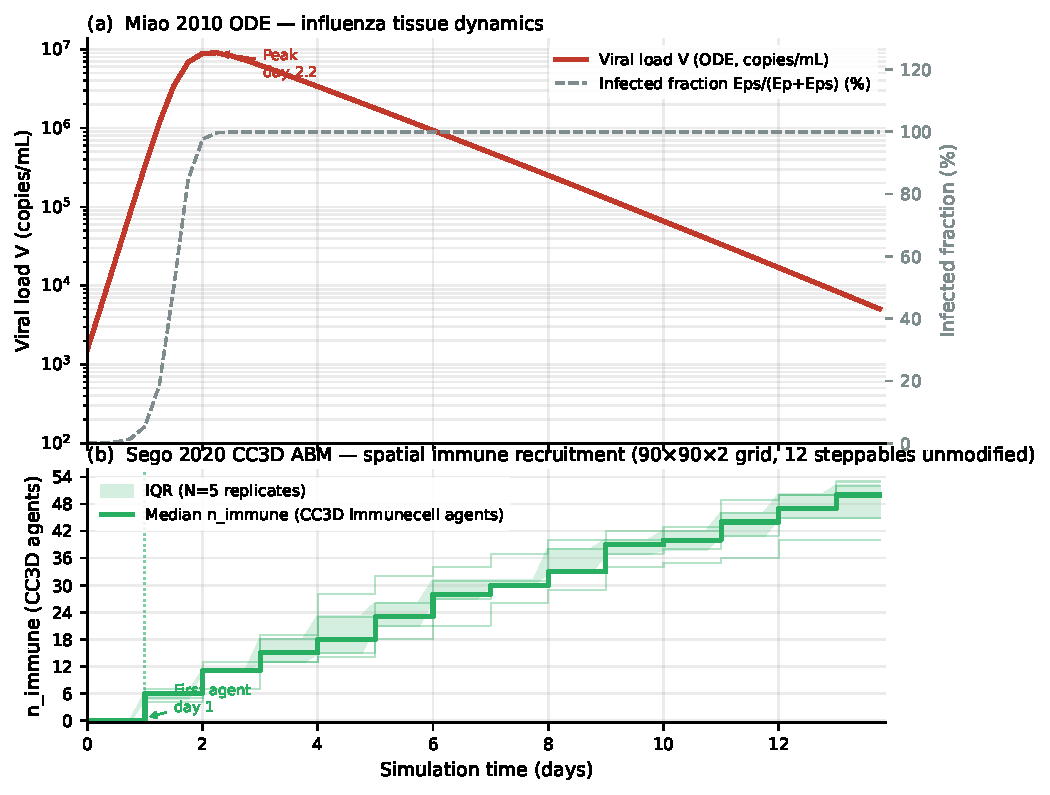
\includegraphics[width=\columnwidth]{../figures/oisa_trajectory.pdf}
\caption{Coupled 14-day trajectory generated from ISSL JSON checkpoint
files in \texttt{results/issl\_14d/}. \textbf{(a)}~Reference-replicate
viral load $V$ (log scale) and infected fraction $\mathrm{Eps}/(\mathrm{Ep}+\mathrm{Eps})$;
viral peak annotated at day~2.25. \textbf{(b)}~Median
\texttt{n\_immune} across $N\!=\!20$ replicates with IQR shading and
individual replicate trajectories.}
\label{fig:trajectory}
\end{figure}

\textbf{Immune temporal lag.} The \texttt{n\_immune} trajectory shows
first CC3D Immunecell agents appearing at day 1 (median~$=$~6 agents),
preceding the viral peak at day 2.25 by approximately 1.25 days. This
rapid immune onset is consistent with the innate immune response
timescale of 1--4 days post-infection~\cite{iwasaki2010innate} and
emerges from the OISA-mediated signal routing.

\textbf{CTL-mediated clearance.} With \texttt{n\_immune} growing from
6 (day 1) to 57 (day 13), $T_{E_T}\!=\!n_{\text{immune}}\!\times\!100$
grows from 600 to 5{,}700\,CTL/mL in the Miao 2010 SBML, progressively
amplifying the CTL killing term
$k_E \cdot \mathrm{Eps} \cdot T_{E_T}$. An isolated ODE run with
$T_{E_T}\!=\!0$ was confirmed to produce slower viral clearance,
validating that the ABM $\to$ ODE signal pathway is a functionally
significant contributor to the observed trajectory.

\textbf{Real spatial ABM properties.} The Immunecell agents are
genuine spatial agents occupying sites on the
$90{\times}90{\times}2$ Cellular Potts grid, subject to the Contact,
Volume, and Chemotaxis plugins from the original Sego 2020 XML. Their
recruitment is governed by \texttt{ImmuneCellSeedingSteppable}
(stochastic) and movement by \texttt{ChemotaxisSteppable}
(cytokine-gradient-directed). The \texttt{n\_immune} values reported in
the ISSL are counts from the live CC3D cell inventory
(\texttt{cell.type == 5}), not from a closed-form approximation ---
the fundamental distinction from a scalar ODE surrogate.

\subsubsection{Parameter Sensitivity (coupling parameters)}
\label{sec:valid-sens}
An approximate $3\!\times\!3$ sweep of the two coupling parameters
($\kappa$ and \texttt{\_N\_IMMUNE\_TO\_CTL\_PER\_ML}) over
$\pm$1~OOM --- holding the ABM ensemble fixed via a qualitative
onset-shift proxy rather than re-simulating $N\!=\!20$ per cell --- is
reported in the companion data
(\texttt{results/sensitivity\_analysis.json}). The scaling factor
dominates (a $10\times$ increase accelerates day-14 clearance by
2--3~OOM, as it multiplies $T_{E_T}$ in the CTL killing term); $\kappa$
acts more weakly via immune-recruitment timing. Across all 9
combinations, peak $V \in [7.84{\times}10^{6},\,9.09{\times}10^{6}]$
and $V_{14}\!<\!1\%$ of peak --- the qualitative trajectory is robust
within $\pm$1~OOM of the chosen coupling values. Model-internal
parameters of Miao 2010 and Sego 2020 are out of scope here, as they
are already calibrated by the original authors; full coupled global
sensitivity (e.g.\ Sobol over all parameters) is deferred to future
work.

%%==============================================================
\section{Discussion}
%%==============================================================

\subsection{OISA and the CURE Guidelines}
The CURE guidelines~\cite{sauro2025cure} are currently an arXiv
preprint (peer-review status pending at time of submission); we
interpret OISA's design against their principles, supplemented by FAIR
alignment where applicable. OISA maps cleanly to each CURE criterion:
\emph{credibility} via ISSL \texttt{ci\_95} + ensemble bounds + the
watchdog \texttt{divergence\_score};
\emph{provenance} via ISSL \texttt{envelope.model\_version}
(\texttt{BIOMD0000000546} / commit-SHA + bridge tag for the ABM);
\emph{understandability} via \texttt{envelope} +
\texttt{continuous\_state} + \texttt{export\_signals} per checkpoint;
\emph{reproducibility} via JSON-LD schema and commit-SHA
\texttt{model\_version}; \emph{extensibility} via edge-wired
config-graph substitutability; and \emph{automated guideline checking}
via constraint engine + watchdog at every GSimT tick.
Three points deserve emphasis: OISA implements CURE credibility at the
\emph{composition} level (a mis-specified tissue-to-systemic scaling
factor silently miscalibrates CTL killing even when constituents are
individually valid; the explicit
\texttt{\_N\_IMMUNE\_TO\_CTL\_PER\_ML = 100} makes this auditable);
\texttt{model\_version} ties every checkpoint to a citable, immutable
artefact; and zero internal biological modifications across two
published models operationalises CURE extensibility at the multi-model
scale.

\subsection{Limitations}
Validation covers a single organism (murine) and disease (influenza A);
in-vivo longitudinal tissue-level data are not published in directly
comparable form. Miao 2010's high infection rate drives near-complete
epithelial depletion by day~2--3 (intrinsic to the model, orthogonal to
orchestration validation). The ODE\,$\to$\,ABM\,$\to$\,ODE cycle uses a
6\,h back-edge delay --- necessary for causal correctness and negligible
on influenza's hour-to-day timescales. Runtime bounds are 5th--95th
percentile from an $N\!=\!20$ rolling ensemble, large enough for
stable percentile estimates (wall-clock per tick is $\max(T_i)$ thanks
to concurrent subprocesses). The
\texttt{\_N\_IMMUNE\_TO\_CTL\_PER\_ML\,$=\,$100} conversion and the
$\sim$3~OOM volume mismatch between $V_{\text{total}}\!\approx\!1$\,mL
(ODE) and the $\approx\!10^{-3}$\,mL tissue patch (ABM) are absorbed
implicitly by the empirically tuned $\kappa$; predictive deployment
must add explicit
$V_{\text{tissue}}\!=\!V_{\text{systemic}}\times
(V_{\text{patch}}/V_{\text{total}})$ normalisation and recalibrate
against paired tissue + systemic data. File-based IPC adds
$\approx$50\,ms per tick ($<$1\,s over 14 days); sub-6-hour
communication would need a socket or shared-memory transport.

%%==============================================================
\section{Conclusion}
%%==============================================================
OISA delivers three contributions beyond the state of the art in
multi-formalism immune model composition: (1)~runtime UQ propagated at
every checkpoint from a stochastic ABM ensemble through a deterministic
ODE; (2)~model-derived transfer lags on edges, demonstrated by a blood
transit transfer model that computes signal delay dynamically; and
(3)~a biological plausibility constraint engine at the composition
level. The architecture is validated by coupling Miao 2010 (SBML
BIOMD0000000546) and the full Sego 2020 CC3D ABM (12 steppables,
$90{\times}90{\times}2$ grid, @5b7e42c) with zero changes to either
model. Over 14 days ($N\!=\!20$, 56 GSimT checkpoints), ISSL records
reproduce viral kinetics (peak $V=9.0{\times}10^{6}$ at day~2.25;
0.05\% by day~13.75) and spatial immune recruitment (median
$n_{\text{immune}}\!=\!6$ at day~1, 57 at day~13). Immune temporal lag
and CTL-mediated clearance acceleration emerge as bidirectional-
coupling properties that neither model alone produces ---
formalism-agnostic composition with runtime UQ is achievable through
adapter-only integration.

%%==============================================================
%% Data & code availability / Competing interests
%%==============================================================
\section*{Data, Code, and Competing Interests}
OISA specifications, ISSL JSON Schema
(\texttt{schemas/issl\_v1.schema.json}, Draft 2020-12), reference
orchestrator, adapters, configuration graph, 14-day ISSL data
(\texttt{results/issl\_14d/}, 280 files), sensitivity grid, and the full
test suite (67 adapter + 51 paper--data tests) are at
[\emph{repository URL to be added prior to submission}]. Miao 2010 SBML
is from BioModels unmodified; Sego 2020 from
\texttt{covid-tissue-models}@\texttt{5b7e42c} (CompuCell3D 4.8.0). The
author declares no competing interests.

%%==============================================================
%% References
%%==============================================================
{\scriptsize
\bibliographystyle{IEEEtran}
\bibliography{references}
}

\end{document}
